\section{Conclusion}

\begin{frame}{Conclusion}
The Abjad API for Formalized Score Control extends the Python programming
language with an open-source, object-oriented model of common-practice music
notation that enables composers to build scores through the aggregation of
elemental notation objects.
\end{frame}

\begin{frame}{Online presence}
    \begin{block}{Documentation}
        http://projectabjad.org
    \end{block}
    \begin{block}{GitHub Repository}
        http://github.com/Abjad/abjad
    \end{block}
    \begin{block}{User Mailing List}
        http://groups.google.com/group/abjad-user
    \end{block}
\end{frame}

\begin{frame}{TENOR 2015 (github.com/Abjad/tenor2015)}
    \begin{figure}
    \begin{centering}
    \begin{tabular}{cc}
    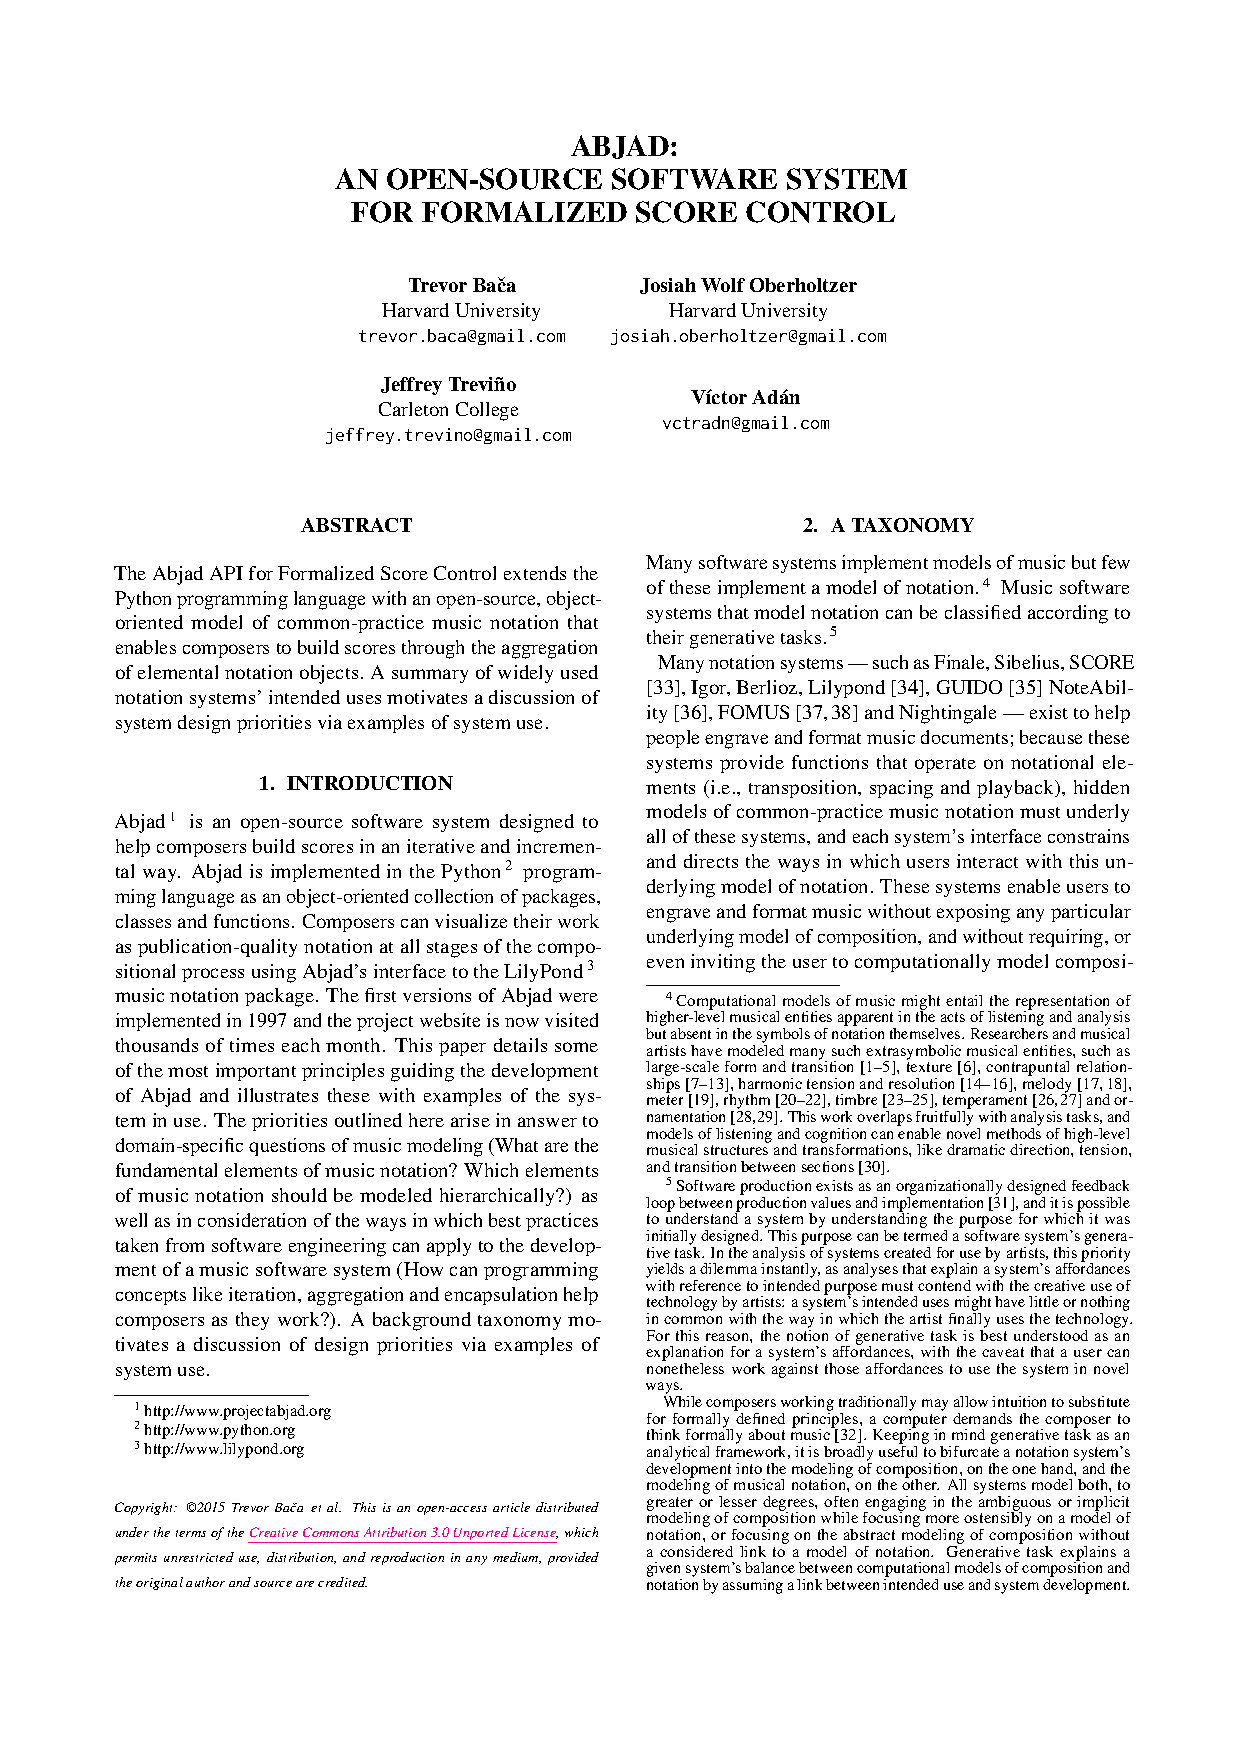
\includegraphics[
        page=1,
        scale=0.2,
        clip=true,
        fbox,
    ]{assets/include-tenor2015.pdf}
    &
    \includegraphics[
        page=2,
        scale=0.2,
        clip=true,
        fbox,
    ]{assets/include-tenor2015.pdf}
    \end{tabular}
    \caption{First International Conference on
        Technologies for Music Notation and Representation,
        May 2015, Paris, France}
    \end{centering}
    \end{figure}
\end{frame}

\begin{frame}{Personal Contacts}
    \begin{columns}[t,onlytextwidth]
        \column{.5\textwidth}
        \textbf{Trevor Ba\v{c}a}
        \begin{itemize}
            \item trevor.baca@gmail.com
            \item trevorbaca.com
            \item github.com/trevorbaca
        \end{itemize}
        \column{.5\textwidth}
        \textbf{Jeffrey Trevi\~{n}o}
        \begin{itemize}
            \item jeffrey.trevino@gmail.com
            \item jeffreytrevino.com
            \item github.com/jefftrevino
        \end{itemize}
    \end{columns}
    \vspace{\baselineskip}
    \textbf{Josiah Wolf Oberholtzer}
    \begin{itemize}
        \item josiah.oberholtzer@gmail.com
        \item josiahwolfoberholtzer.com
        \item github.com/josiah-wolf-oberholtzer
    \end{itemize}
\end{frame}